\section{Background and Related Works}
\label{sec_related}

\begin{enumerate}
\item Brief architecture of FPGAs
\item Previous hardware implementations
\end{enumerate}


\begin{figure}[t]
\centering
   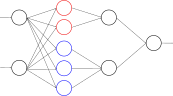
\includegraphics[height=0.6\columnwidth]{Figures/pnn.pdf}
   \caption{General layered architecture of PNN}
   \label{fig:pnn}
\end{figure}

Probabilistic Neural Network (PNN) is a feed forward artificial neural networks developed for solving classification problems \cite{specht1990}.
During network training, PNN stores the statistical parameters of the training data and later uses this information to classify the inputs.
PNNs have been successfully used in applications such as human emotion \cite{zhang2016pnn} and speech recognition \cite{wrobel2017}, biometric identification \cite{junjea2015}, intrusion detection in IT infrastructure \cite{raman2017,zhao2017}, medical diagnos etc.~\cite{mangayarkarasi2017,thara2016}.


The general architecture of a PNN is as shown in Fig.~\ref{fig:pnn}.
It has a layered structure consisting of input layer, pattern layer, summation layer, and output layer. 
The input layer is responsible for receiving the data to be classified. 
Each data item is represented as a feature vector (p features in the example).
The pattern layer consists of multiple groups of neurons each group representing one class for classification (two classes in the example).
During training, the weight vector of each pattern neuron $W$ is set to be equal to the features of the corresponding training sample $X$.
Thus each neuron in the pattern layer represents a training sample.
Each input layer neuron is connected with every pattern layer neuron with different weights assigned to the connection. 
The pattern neurons perform dot product between input vector $X$ and weight vector $W$ and applies the result to an activation function. 
Traditional PNNs employ exponential based activation for classification, where the output of $i$th pattern neuron $g_i$ is expressed as Eq. 1 \cite{specht1988}.

\begin{equation}
g_{i}=\frac{1}{\sqrt{2\pi\sigma^{2}}}exp\left(\frac{\boldsymbol{X\cdot W_{i}}-1}{\sigma^{2}}\right)
\end{equation}

Here $\sigma$ is a smoothing parameter, which defines the probability density function (PDF) of the data class. 
Selection of $\sigma$ parameter affects the accuracy of the classification and is generally selected based on heuristic algorithms.
The summation layer, adds and averages the outputs of pattern neurons belonging to each class to produce the probability distribution of this class. 
Finally, the output layer chooses the class with the highest probability as the class of the input sample.


PNNs have the advantages of much faster training process and more accurate results using the minimum Bayesian risk criterion compared with other networks, such as multilayer perceptron networks.
They are faster since the PNNs weights are not \emph{trained} but rather assigned.
In software implementations, PNN requires larger memory for storing the model since the features corresponding to every training data has to be stored and one neuron per train data is required to process the input.
Moreover, as the number of training set increases, the system will need to perform more computation resulting in decrease in speed of classification. 



\cite{Zhou2010,Figueiredo1998,Ovtcharov2015,Zhu2010,Shima2007,Bu2004,Zhang2015}